\documentclass[12pt]{article}

\usepackage[T1]{fontenc}
\usepackage[utf8]{inputenc}
\usepackage{natbib}
\usepackage[french]{babel}
\addto{\captionsfrench}{\renewcommand{\refname}{Références}}
\usepackage[labelfont=bf, justification=centering]{caption}
\usepackage{graphicx}
\usepackage{lettrine}
\usepackage{mathptmx}
\usepackage{fancyhdr}
\renewcommand{\LettrineTextFont}{\normalfont}

\fancypagestyle{plain}{
  \fancyhf{}
  \fancyhead[]{}% Right header
  \fancyfoot[]{}% Left footer
  \fancyfoot[R]{\thepage} % Right footer
}
\pagestyle{plain}

\title{\textbf{L’impact de la COVID-19 sur les réseaux des étudiants du cours BIO500 à l’hiver 2021}}

\author{Coralie Godon \\ Ève Lapointe \\ Anne Ju Laberge \\ Anaïs Nappert Drouin \\ \small Dans le cadre du cours \\ BIO500}
\date{\small 25 Avril 2021}



\begin{document}
\maketitle
\begin{abstract}
    Le coronavirus a bouleversé le monde entier depuis son apparition. Les universités n’y ont pas échappé et ont dû faire une grande réorganisation de leurs activités, entre autres en ce qui concerne les travaux d’équipe. Nous nous sommes intéressés à l’effet de la pandémie sur les réseaux de collaborations des élèves du cours Méthode en écologie computationnelle (BIO500) à l’hiver 2021. Nous avons pu observer 796 collaborations avant la pandémie et 414 après. Le réseau post-covid est ainsi beaucoup plus restreint. Nous croyons que les mesures sanitaires ont fait réduire les relations des étudiants en termes de collègues d’équipe et que le nombre de travaux d’équipe a aussi été réduit par les professeurs. 

\end{abstract}
\hspace{4cm}

\section*{\large Introduction\vspace{-0.1cm}}
En mars 2020, le Québec s’est arrêté à la suite de l’apparition du coronavirus. Ce virus ayant envahi le monde entier a beaucoup bouleversé le milieu universitaire \citep{Gouvernement}. Par exemple, les activités de groupes, les sorties terrain, et les travaux d’équipes n’ont pas pu se dérouler comme prévu \citep{UniversiteShebrooke2021}. La propagation exponentielle du virus illustre bien les réseaux des individus \citep{komarova_patterns_nodate}. Ainsi, nous nous sommes intéressées aux modifications dans le réseau de collaborations des étudiants du cours Méthode en écologie computationnelle (BIO500) à l’hiver 2021 en contexte de pandémie. La situation de Covid-19 a-t-elle affecté la composition des équipes dans les cours en présentiel et à distance? Les étudiants ont-ils restreint leur réseau dû à l’enseignement à distance?
\par Afin de visualiser et comprendre comment les cours à distance ont pu influencer les travaux d’équipe, nous avons établi un réseau comportant toutes les collaborations que les étudiants du cours ont eues depuis le début de leur baccalauréat. Nous avons ensuite créé un réseau montrant les différentes collaborations entre étudiants pendant la période pré-covid et un autre pendant la période covid. Suite à la création de ces réseaux, nous avons créé un tableau comparatif illustrant le nombre de collaborations par session.

\section*{\large Méthodologie\vspace{-0.1cm}}
D’abord, tous les étudiants de BIO500 ont rempli 3 fichiers selon les informations demandées. Le groupe était divisé en deux et les fichiers ont été remplis avec les informations et normes décidées dans chaque sous-groupe. Nos trois fichiers représentaient: 
\par – Les nœuds : noms des étudiants, session de début, leur programme, leur participation au programme coop et leur participation au cours BIO500.
\par – Les cours : sigle des cours, nombre de crédits, s’ils ont été donnés en présence ou non et le choix libre ou non des équipes dans ces cours.
\par – Les collaborations : chaque collaboration entre les étudiants, le cours et la session de leur collaboration. 
\par Avant la réalisation des différentes étapes, les paquets suivants ont été installés sur le logiciel Rstudio : dplyr \citep{wickham2021}, RSQLite \citep{muller2021}, igraph \citep{csardi2006}, reshape2 \citep{wickam2007}.

\subsection*{\small Bases de données\vspace{-0.1cm}}
La première étape fut d’importer les 3 fichiers «.csv» de chaque équipe de notre sous-groupe dans le logiciel RStudio sous forme de listes. L'uniformisation des noms des colonnes a été assurée avec la commande «rename». L’une des listes «noeuds» comportait seulement 4 colonnes, plutôt que 5. Nous avons donc ajouté la colonne «BIO500» manquante avec les fonctions de création de vecteurs et «as.integer». Puis, nous avons combiné toutes les listes de chaque équipe ensemble avec la fonction «bind.rows», formant 3 listes principales «nœuds», «cours» et «collaboration». 
\par Ensuite, nous avons procédé au nettoyage de chaque liste séparément avec différentes fonctions. Nous avons utilisé la commande «sort(unique())» pour visualiser les données uniques et nous assurer de leur uniformisation. En cas d’erreurs, nous les avons corrigées. Nous avons ensuite enlevé les doublons présents en utilisant la commande «duplicated» dans chaque liste. Nous avons finalement enregistré 3 bases de données pour les nœuds (data\_noeuds), les cours (data\_cours) et les collaborations (data\_collab).

\subsection*{\small Les figures \vspace{-0.1cm}}
Pour la création des figures, il a d’abord fallu créer trois tables avec le langage SQL, soit «nœuds», «cours» et «collab», en utilisant «CREATE TABLE». Ensuite, nous avons injecté les 3 bases de données créées dans chacune des tables correspondantes avec «dbWriteTable». Puis, nous avons fait les requêtes nécessaires avec le langage SQL pour répondre à nos questions, la première pour le réseau de toutes les collaborations entre les étudiants, la deuxième pour les collaborations pré-covid, la troisième pour les collaborations post-covid et la quatrième pour générer un tableau des collaborations en fonction des sessions.
\par Pour créer les figures, nous avons utilisé le package «igraph». Pour chaque figure créée, nous avons utilisé les fonctions «subset» et «acast» pour créer des matrices carrées qui ont ensuite été utilisées dans la fonction «graph.adjacency». Avec cette dernière fonction, nous avons créé un objet qui permet de visualiser les réseaux avec la fonction «plot». La fonction «simplify» a été utilisée afin de simplifier l’objet et enlever les boucles notamment. 

\section*{\large Résultats\vspace{-0.1cm}}
Dans cette section, nous présentons les trois réseaux qui représentent les collaborations entre les étudiants du cours Méthode en écologie computationnelle (BIO500) à l’hiver 2021 au total, avant les mesures pandémiques (pré-covid: H18, A18, H19, A19, H20, voir tableau 1 pour les codes des noms des sessions) et après les mesures pandémiques (post-covid: E20, A20, H21), ainsi que le tableau sur le nombre de collaborations classé par session. Les collaborations représentent les liens entre les élèves du cours et leurs collègues lors de travaux d’équipe depuis leur entrée à l’université. 
\par La figure \ref{fig1} illustre le réseau de l’ensemble des collaborations des étudiants. Le gradient des tailles des nœuds représente le nombre d’interactions faites par étudiant. Les petits cercles ont une valeur de 1 et les plus grands cercles ont une valeur de 11. 

\par La figure \ref{fig2} illustre le réseau des collaborations des étudiants pré-covid. Le même gradient de taille des nœuds est présent ici, donc les petits cercles ont une valeur de 1 et les plus gros cercles ont une valeur de 7. 

\par La figure \ref{fig3} illustre le réseau des collaborations des étudiants en période covid. Un gradient de taille des nœuds est aussi présent ici, mais les petits cercles ont une valeur de 1 et les plus gros cercles ont une valeur de 6.

\par Le tableau \ref{tableau} représente le nombre de collaborations présentes chaque session de la base de données. Pour les sessions pré-covid, le total de collaborations monte à 796, alors que pour les sessions en période covid, le total est de 414 collaborations.

\begin{figure}
    \centering
    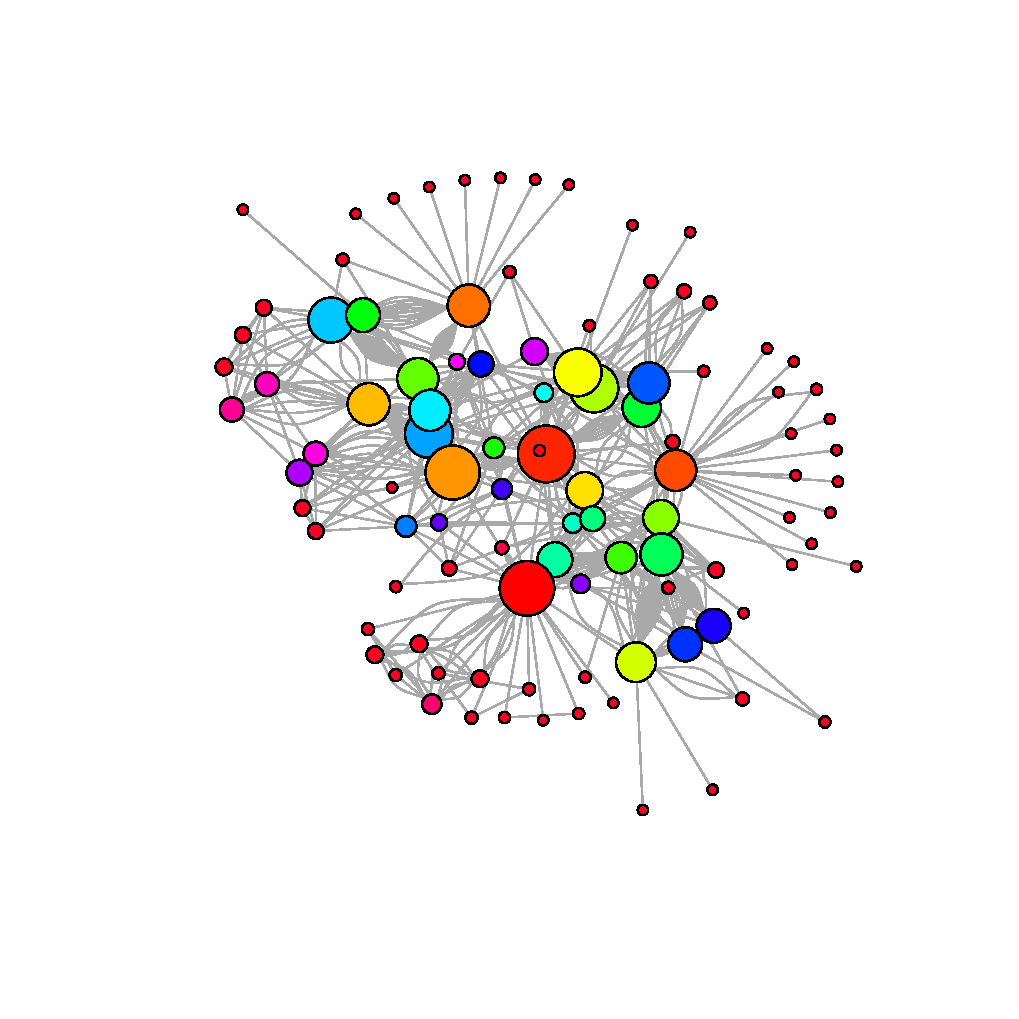
\includegraphics[width=1\textwidth]{figures/fig1.pdf}
    \caption{Réseau de collaborations des étudiants du cours Méthode en écologie computationnelle (BIO500) à l’hiver 2021. Plus petits cercles : 1 collaboration, plus grands cercles : 11 collaborations}
    \label{fig1}
\end{figure}

\begin{figure}
    \centering
    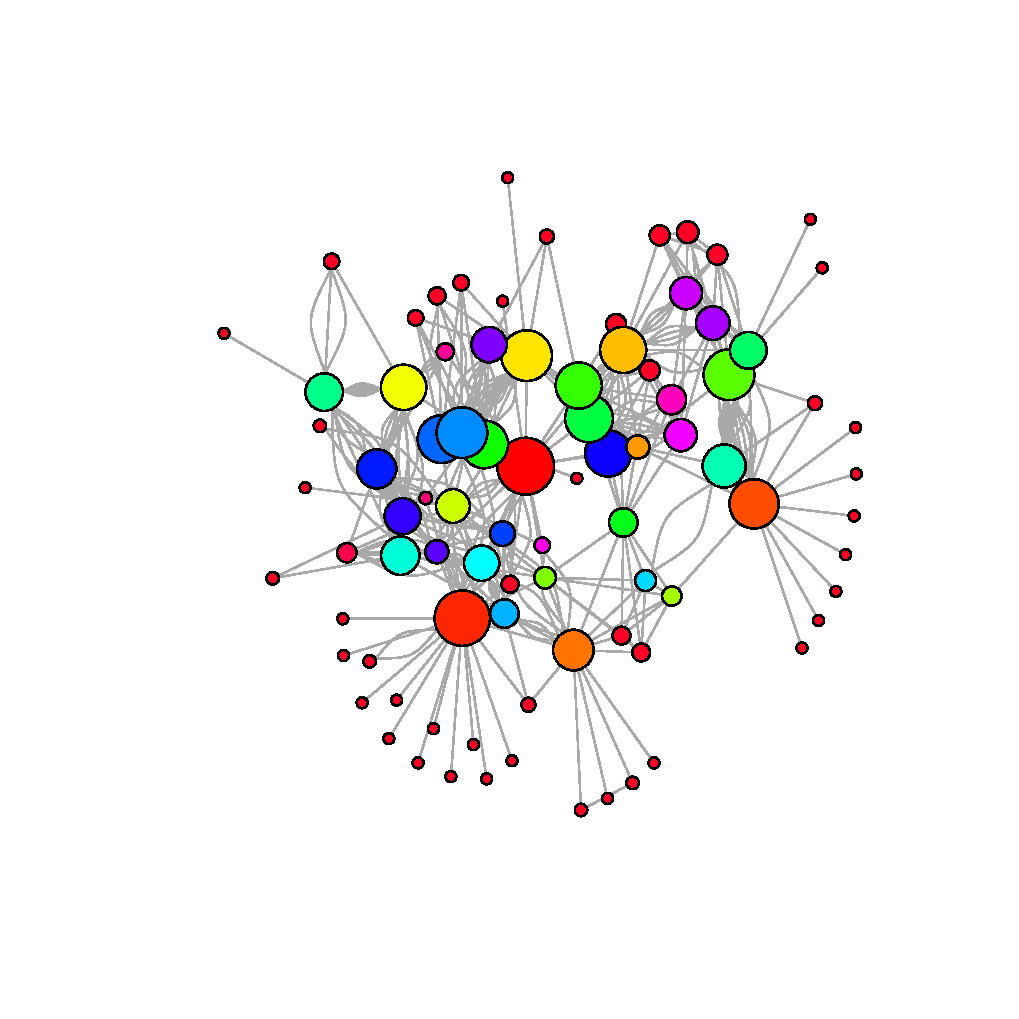
\includegraphics[width=1\textwidth]{figures/fig2.pdf}
    \caption{Réseau de collaborations pré-covid des étudiants du cours Méthode en écologie computationnelle (BIO500) à l’hiver 2021. Plus petits cercles : 1 collaboration, plus grands cercles : 7 collaborations}
    \label{fig2}
\end{figure}

\begin{figure}
    \centering
    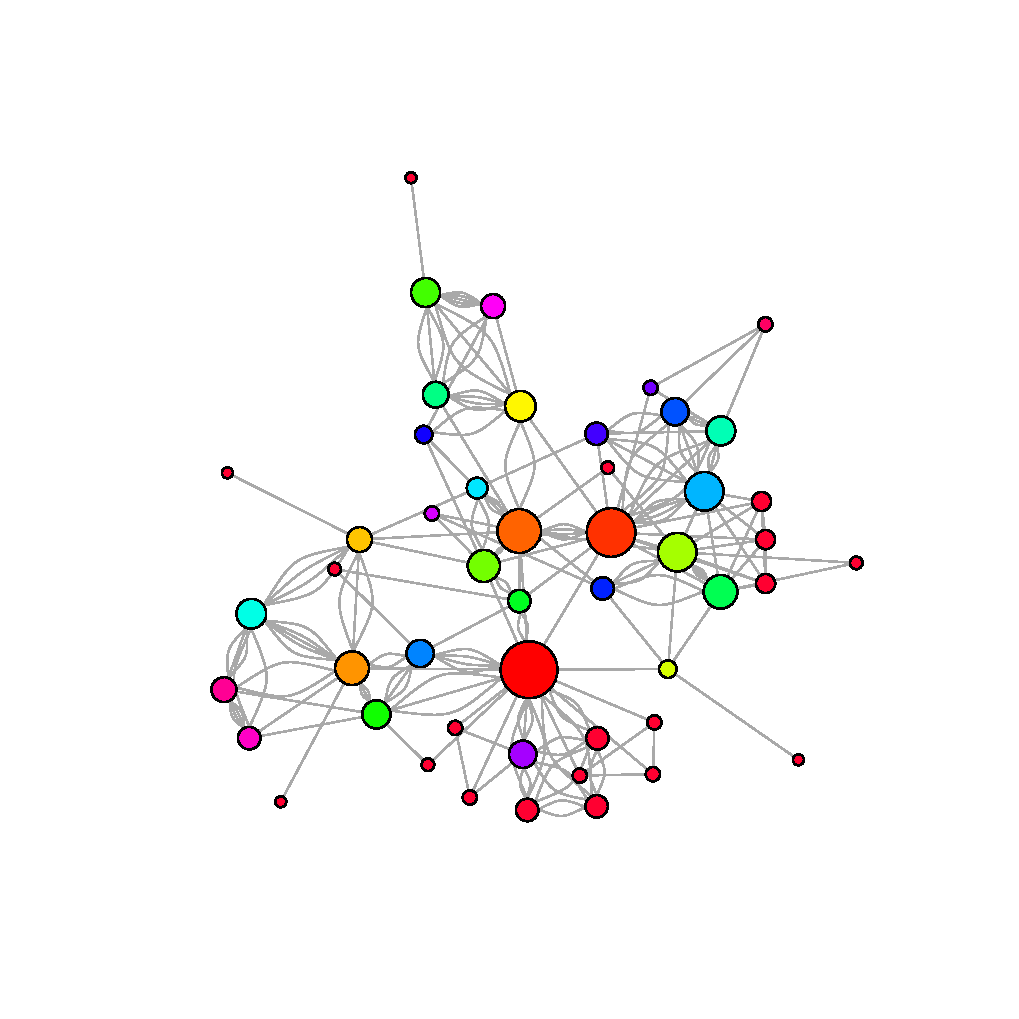
\includegraphics[width=1\textwidth]{figures/fig3.pdf}
    \caption{Réseau de collaborations en période covid des étudiants du cours Méthode en écologie computationnelle (BIO500) à l’hiver 2021. Plus petits cercles : 1 collaboration, plus grands cercles : 6 collaborations}
    \label{fig3}
\end{figure}

\begin{table}
    \centering
    \begin{tabular}{c|c}
    Session & Nombres de collaborations \\
    \hline
    H18 & 16 \\
    A18 & 4 \\
    H19 & 537 \\
    A19 & 233 \\
    H20 & 6 \\
    E20 & 130 \\
    A20 & 98 \\
    H21 & 186
    \end{tabular}
    \caption{Nombre de collaborations en fonction des sessions des étudiants du cours Méthode en écologie computationnelle (BIO500). Les noms des sessions suivent les codes suivants : A: Automne, H: Hiver, E: Été, 18:2018, 19:2019, 20:2020, 21:2021}
    \label{tableau}
\end{table}

\section*{\large Discussion\vspace{-0.1cm}}
Les réseaux représentant les collaborations entre étudiants des sessions avant et pendant la covid diffèrent. En effet, le réseau pré-covid \ref{fig2} comporte moins de liens que le réseau depuis le début de la covid \ref{fig3}. Le tableau \ref{tableau} permet d’observer cette différence, les sessions pré-covid totalisent 796 collaborations et celles depuis la covid comptent 414 collaborations. 
\par On pourrait penser que le nombre de collaborations est plus élevé pour la période pré-covid puisqu’en somme il y a plus de sessions comprises dans cette période. Or, on peut voir dans le tableau \ref{tableau} que beaucoup de celles-ci possèdent seulement quelques liens, par exemple H18 et A18 qui totalisent 20 collaborations. En effet, les collaborations incluses dans ces sessions sont souvent celles d’élèves à parcours particuliers. Ainsi, si nous les retirons, nous nous retrouvons avec un même nombre de sessions pour la période pré-covid, soit H19, A19 et H20 (774 collaborations), que la période pendant la covid, soit E20, A20, H21 (414 collaborations). Le nombre de collaborations reste beaucoup plus élevé pour la période pré-covid.
\par Même si l'ensemble des cours dans la période pendant la covid étaient offerts en ligne, certains projets ont impliqué la formation d’équipe. Nous pensons que, dû aux règlements sanitaires et des inquiétudes face à la pandémie, plusieurs étudiants ont probablement préféré restreindre leurs collaborations aux amis proches. La communication et la création d’équipe à distance sont donc facilitées. Lors de cours présentiels, les équipes sont parfois formées selon la disposition des élèves dans la classe, ou selon la décision de l’enseignant. Voilà ce qui pourrait expliquer la divergence entre les réseaux. 
\par Une autre raison de la diminution du nombre de collaborations depuis la covid pourrait être que les professeurs, en changeant leur méthode d’enseignement, ont demandé davantage de travaux individuels qu’en équipe. En effet, à l’Université de Sherbrooke, des mesures sanitaires spéciales ont été mises en place demandant aux professeurs de diminuer le nombre d’activités académiques en équipe pour réduire la propagation du virus \citep{UniversiteShebrooke2021}. 
\par Pour notre travail, nous avons éprouvé de nombreuses difficultés à respecter une forme standard pour la saisie de données entre chaque équipe. Malgré le consensus initial, beaucoup de détails ont été échappés. La standardisation de la collecte d’information est une étape cruciale dans une collaboration où plusieurs étudiants participent à la collecte des données \citep{desquilbet_vers_2019}. Une révision collective de la base de données aurait pu être faite pour s’assurer de son uniformisation \citep{baker2016}. La mise en commun des données de chaque équipe nous a fait prendre conscience du défi que représente le partage de données dans le domaine de la recherche et l’importance d’être rigoureux et constant dans toutes les étapes de l’expérience.

\section*{\large Conclusion\vspace{-0.1cm}}
Les résultats obtentenus illustrent une dissimilarité entre les réseaux de collaborations des étudiants avant la pandémie et depuis la pandémie. Le nombre de collaborations dans les cours en présence est plus élevé que dans les cours à distance, probablement dû au fait que les normes sanitaires ont restreint les interactions entre élèves, traduit par un nombre inférieur de travaux d’équipe, et des collaborations moins diversifiées. Il serait toutefois intéressant de faire des analyses plus poussées avec ce jeu de données afin de démontrer si la relation entre les collaborations pré-covid et post-covid illustrées est significative ou non, afin d’établir un vrai effet de causalité au lieu de spéculations comme nous avons fait dans ce travail.


\nocite{*}
\bibliographystyle{apalike}
\bibliography{ref}

\end{document}
